\documentclass[13pt]{ctexart}
\usepackage{geometry}
\usepackage{graphicx}
\renewcommand{\figurename}{Figure}
\renewcommand{\tablename}{Table}
\renewcommand{\contentsname}{Contents}
\usepackage{changepage}
\usepackage{fontspec}
\usepackage{fancyhdr}
\usepackage{graphicx}
\usepackage{subfigure}
\usepackage{overpic}
\pagestyle{fancy}
\usepackage[shortlabels]{enumitem}
 \usepackage{amsmath} 
 \usepackage{amssymb}
\usepackage{titlesec}
\titleformat*{\section}{\LARGE}
\titleformat*{\subsection}{\Large}
\titleformat*{\subsubsection}{\Large}
\usepackage{amsmath}
\usepackage{array}
\usepackage{booktabs}
\usepackage{etoolbox}
\patchcmd{\thebibliography}{\section*{\refname}}{}{}{}
\usepackage{url}
\setmonofont{IBM Plex Mono}
\usepackage{xcolor}
\usepackage{listings}
\definecolor{CPPLight}  {HTML} {686868}
\definecolor{CPPSteel}  {HTML} {888888}
\definecolor{CPPDark}   {HTML} {262626}
\definecolor{CPPBlue}   {HTML} {4172A3}
\definecolor{CPPGreen}  {HTML} {487818}
\definecolor{CPPBrown}  {HTML} {A07040}
\definecolor{CPPRed}    {HTML} {AD4D3A}
\definecolor{CPPViolet} {HTML} {7040A0}
\definecolor{CPPGray}  {HTML} {B8B8B8}
\lstset{
	basicstyle=\ttfamily,
	breaklines=true,
	framextopmargin=50pt,
	frame=bottomline,
	columns=fixed,       
    %numbers=left,                                       % 在左侧显示行号
	frame=none,                                          % 不显示背景边框
	backgroundcolor=\color[RGB]{255,255,255},            % 设定背景颜色
	keywordstyle=\color[RGB]{40,40,255},                 % 设定关键字颜色
	numberstyle=\footnotesize\color{darkgray},           % 设定行号格式
	commentstyle=\itshape\color[RGB]{0,96,96},                % 设置代码注释的格式
	stringstyle=\slshape\color[RGB]{128,0,0},   % 设置字符串格式
	showstringspaces=false,                              % 不显示字符串中的空格
	language=python,                                     % 设置语言
	morekeywords={alignas,continute,friend,register,true,alignof,decltype,goto,
		reinterpret_cast,try,asm,defult,if,return,typedef,auto,delete,inline,short,
		typeid,bool,do,int,signed,typename,break,double,long,sizeof,union,case,
		dynamic_cast,mutable,static,unsigned,catch,else,namespace,static_assert,using,
		char,enum,new,static_cast,virtual,char16_t,char32_t,explict,noexcept,struct,
		void,export,nullptr,switch,volatile,class,extern,operator,template,wchar_t,
		const,false,private,this,while,constexpr,float,protected,thread_local,
		const_cast,for,public,throw,std},
	emph={map,set,multimap,multiset,unordered_map,unordered_set,numpy,graph,path,append,extend,
		unordered_multiset,unordered_multimap,vector,string,list,deque,
		array,stack,forwared_list,iostream,memory,shared_ptr,unique_ptr,
		random,bitset,ostream,istream,cout,cin,endl,move,default_random_engine,
		uniform_int_distribution,iterator,algorithm,functional,bing,numeric,},
	emphstyle=\color{CPPViolet}, 
}

\begin{document}
\newgeometry{top = 1cm, right = 2.54cm, left = 2.54cm, bottom = 2.54cm}
% 第一页的字体为times new roman
\setmainfont{Times New Roman}
\thispagestyle{empty}

\begin{table}[h]
    \quad { }  \begin{minipage}[t]{5.5cm}
        % arraystretch 是调节列高
        \begin{tabular}[t]{>{\centering\arraybackslash}b{10em}}
            \fontsize{12pt}{10pt}\selectfont \textbf{Problem Chosen}\\ [2pt]
            {\color{red} \fontsize{20pt}{10pt}\selectfont C}
        \end{tabular}
    \end{minipage}
    \begin{minipage}[t]{5.2cm}
        \begin{tabular}[t]{>{\centering\arraybackslash}p{10em}}
            \fontsize{12pt}{10pt}\selectfont \textbf{2021} \\ [-2pt]
            \fontsize{12pt}{10pt}\selectfont \textbf{MCM/ICM} \\ [-2pt]
            \fontsize{12pt}{10pt}\selectfont \textbf{Summary Sheet}
        \end{tabular}
    \end{minipage}
    \begin{minipage}[t]{3cm}
        \begin{tabular}[t]{>{\centering\arraybackslash}b{12em}}
            \fontsize{12pt}{10pt}\selectfont \textbf{Team Control Number} \\ [2pt]
            {\color{red} \fontsize{21pt}{10pt}\selectfont 2111874}
        \end{tabular}
    \end{minipage}
\end{table}
\vspace{-20pt}
\noindent{\rule{\textwidth}{0.5mm}}

% 标题
{\centering\fontsize{18}{16}\selectfont\textbf{{Analyzing the Spread of the Asian Giant Hornet}}
% 摘要
\vspace{1pt} 

\fontsize{13}{10}\selectfont\textbf{{Summary}}\par}

\vspace{10pt}

% 正文字体 13 pt
\fontsize{13}{12.5}\selectfont

\begin{adjustwidth}{1cm}{1cm}
\indent { }{ }{ }{ }{ }{ }Species invasion are always concrened by the people, because it could bring so many severe problems such as breaking the ecological balance and demaging the biodiversity. Here, we discuss a certain insect called Asian Giant Hornet (hornet below), discovered on Canada and propose a model to deal with the relavant problems.
To reveal the severity of the hornet invasion, we constructed a model that simulates the spread of the hornet in Washington State without human intervention.Secondly, aiming at the analysis problem of massive reports, we build a report reliability evaluation system to evaluate the reliability of a report.

In Task 1, we first examine the hornet spread over time, we use ADF method to test the data series stationarity, and found that it is not a smooth time series, at the same time, we calculated the Spearman correlation coefficient of propagation index in time, confirm the spread of hornet and time has a moderate positive correlation.In addition, we divided the target area into small rectangles and used cellular automata to simulate the spread of the hornet, which proved that if nothing was done, the hornet would spread throughout the central and western state of Washington.

In Task 2, we set up a report reliability evaluation system to measure the probability of a report being a positive eyewitness report using a reliability index.We used the analytic hierarchy process (AHP) to select four important indicators through manual selection, namely photo, Dection time, Location and Notes.And their weights are determined by using the positive reciprocal matrix.For photos, CNN is used to evaluate the indicators of images; for Detection Time, statistics and quartic polynomial fitting are used to evaluate the indicators; for Location and Note, the idea of K-nearest neighbor is used to complete the evaluation.And finally, by a weighted sum,
To calculate the reliability, which in turn reflects the probability of the report being misjudged.

In Task 3 to Task 4, we used our report reliability evaluation system to analyze the existing reports, and through screening and mapping, we found the areas where reports with high reliability were enriched, which were the areas for our limited investigation.
Then, we combined computation cost and updating frequency, and discussed a model updating strategy that could continuously improve model accuracy over time without bringing too much computation burden.

In Task 5, we preliminarily discuss the conditions for judging whether an area is free from the threat of the hornet, based on the reported frequency of occurrence and the breeding cycle of the hornet.

\vspace{10pt}
\textbf{key words} : Asian giant hornet; Cellular Automata; ADF; AHF; CNN;
\end{adjustwidth} 

% 开始写 memo 信
% 更换字体为 palatino 也可以不换
\setmainfont{texgyrepagella-regular.otf} 
\newpage
\newgeometry{left = 3.5cm, right = 3.5cm}
\thispagestyle{empty}

{\centering \fontsize{18pt}{14pt}\selectfont \textbf{MEMO}\par}
\noindent Dear Officials:

\vspace{10pt}



Recently, we discovered that a species called the Asian giant hornet has begun to invade Washington state.

To further analyze the severity of the issue, we modeled its spread.
By 2020, the number of reports of suspected Asian giant hornet sightings has increased each year.

Our model suggests that if nothing is done about the Asian giant hornet invasion, the impact could be so dramatic after five years that the ecological and economic losses could be incalculable.
We recommend tracking the insect's movements as soon as possible and taking prompt action to limit the damage.
It is impossible to carry out a comprehensive investigation of this pest with limited resources and manpower.

Relying on people to report suspected targets is a good means of information collection, but because ordinary people do not have the knowledge and experience to collect information on such insects, most of the information reported is chaotic, and it is difficult to conduct accurate analysis.
In addition, it is difficult to process such a huge amount of information with limited manpower.
In this regard, we have established a report reliability assessment system to help filter valuable reporting information, to help you quickly determine whether a sighting report is valid or not.

So far, we have analyzed and evaluated the sightings provided, and made a brief analysis of the temporal and spatial distribution of the reported locations. According to the analysis, hornet sightings are more likely to occur in Bellingham, which can be used as a reference when dispatching commissioners to investigate.

Due to the limited amount of data available, the results of our analysis are incomplete.
However, we have taken this into account, and as soon as we have new data, we can update the model further to achieve better results.
Our model will give the probability index of whether the report is valid or not, and then judge whether to update the model.
If the report can be judged by professionals and then input into the model, the accuracy can be improved.
Given the importance of computational cost and model accuracy, we recommend that departments adopt an update strategy: if there are valid reports, update them immediately; otherwise, update the models with new reports at the end of each month.

The following methods can be used to determine whether the Asian giant hornet has been eliminated:

We consider the month to be safe if reports received within a year from a certain month have reliability predictions below 0.571.
Of course, this could be influenced by chance, but the analysis of the reports so far does not indicate that there is such a chance for six months.
If it is safe for six months in a row, then we can rest assured.

Based on our analysis, we offer some suggestions for controlling the Asian giant hornet:

\begin{enumerate}[1.]
	\item Small survey teams can be sent to investigate areas of high Asian giant hornet density to obtain more detailed and reliable data.
	
	\item On the website receiving the report, it is advocated to use scientific and accurate words for the characteristics of observed insects and briefly introduce the scientific methods of photographing insects. Improving the relevant literacy of the people will help to improve the effectiveness of the report.
	
	\item Timely update the model with time changes to improve the accuracy of the model and track the trend of Asian giant hornet more accurately and timely.
	
	\item A combination of chemical and biological control may be considered. Spraying interferon or other chemicals targeted at the Asian giant hornet in dense nesting areas reduces its population density, and introducing its natural enemies slows its growth.
\end{enumerate}

We believe this model has implications for controlling the effects of the Asian giant hornet. Please contact us for further cooperation.

% 信多出一页,清理页眉页脚
\thispagestyle{empty}
% 信的结尾
\vspace{8.5pt}
{\raggedright
Sincerely yours	\par
FROM: Team \#2111874 \par
Date: Feb. 6, 2021 \par
}

% 目录页
\newpage
\thispagestyle{empty}
\tableofcontents
\newpage
% 目录页后面是第一页
\setcounter{page}{1}

% 开始写正文
% 设置正文的页边距
\newgeometry{top=3cm, left=3.5cm, right=3.5cm}
% 设置正文的页眉页脚
\fancyhf{}
\fancyhead[C]{ }
% 此处修改右上角页码
\fancyhead[R]{Page \thepage\ of 18}
%\fancyhead[R]{Page \thepage\ of 15}
\fancyhead[L]{Team \# 2111874}
\fancyfoot[C]{\bfseries\thepage}

% ----------------------------------------------------
% Section 1
% ----------------------------------------------------

\textbf{\section{Introduction: Assumptions}}

Due to the lack of necessary data, we make the following assumptions to help us perform modeling.
\begin{itemize}[itemsep=0.3ex, leftmargin=1.2cm]
	\item[1.] Asian hornet begin to appear as early as March 1 (the beginning of spring in the northern hemisphere), and all hornets except the queen hornet die as late as December 1 (the beginning of winter in the northern hemisphere).According to the PDF of the question, the hornet is born every year. In the spring, the queen wakes up and begins to look for a place to build a nest. The population grows slowly and peaks in August.
	
	\item[2.] In September, the queen hornet begins to lay eggs, and about 0.35 females are fertilized and then set out to build new nests next year.According to the accompanying PDF, the fertilized females survived and established their hives.
	
	\item[3.] The species is not under very strong control.Within the range predicted by the model, the habitat of Asian hornets was not significantly affected.At the same time, as an invasive species, the Asian hornet is free to breed without having to deal with its natural predators.
	
	\item[4.] The new nest distance of the newly fertilized female wasp obeys the Poisson distribution.
	
	\item[5.] Because the water area is so small, the area containing water is still considered land.
\end{itemize}

%\begin{table}[h]
%	\centering
%	\vspace{3pt}
%	\begin{tabular}{>{\centering\arraybackslash}p{5em}>{\centering\arraybackslash}p{30em}}
%		\toprule % 绘制第一条线
%		Symbol & Meaning \\ \midrule
%		$t$ & Time \\
%		$N$ & Total reported opioid cases\\
%		$N_t$ & Total reported drug cases\\
%		$\lambda$ & Average cases induced by a single case\\
%		$A_t$ & Status at $t$ \\ 
%		$E$ & Set containing socio-economic factors with high correlation $t$ \\
%		$T$ & Transition matrix\\ 
%		$i(t)$ & Proportion of opioid cases in all drug cases at $t$ \\
%		$\mu_1$ & Average number of drug cases induced by an existing drug case \\
%		$\mu_2$ & Number of opioid cases induced among all drug cases \\
%		$\gamma$ & Drug spread slow down factor \\
%		$i_0$ & Status at $t$ \\ 
%		$H$ & Information Entropy \\ 
%		$p_0$ & Initial number of drug cases\\
%		\bottomrule
%	\end{tabular}
%\end{table}

% ----------------------------------------------------
% Section 2
% ----------------------------------------------------

\textbf{\section{Data Processing}}
\textbf{\subsection{Repeated Data Verification}}
According to the PDF description of the title, each global-id is unique and does not have the phenomenon of repetition. The correctness of this information is verified through programming, so there is no need to screen out the duplicate lines.

\begin{figure}[htbp]
	\centering
	\begin{minipage}[t]{0.48\textwidth}
		\centering
		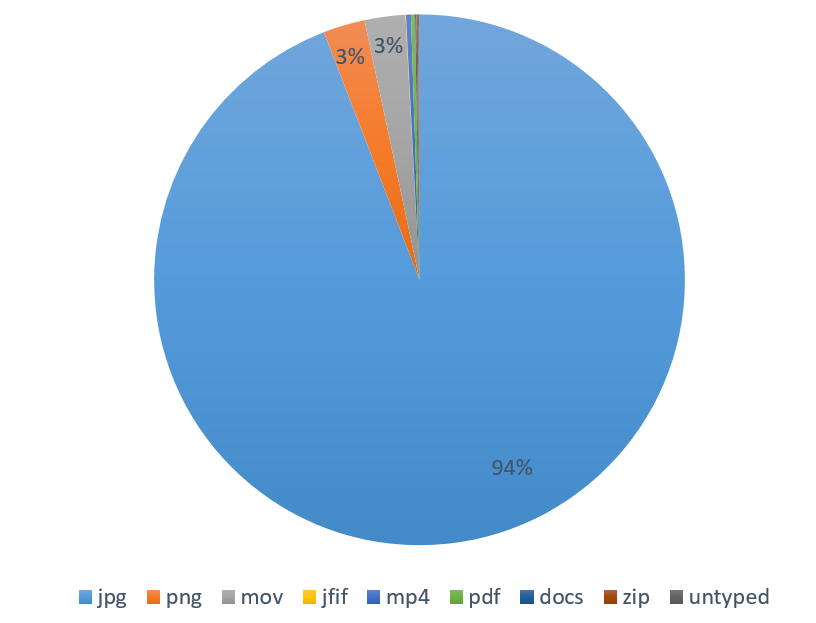
\includegraphics[width=7cm]{images/fan1.png}
		\caption{Files}
	\end{minipage}
	\begin{minipage}[t]{0.48\textwidth}
		\centering
		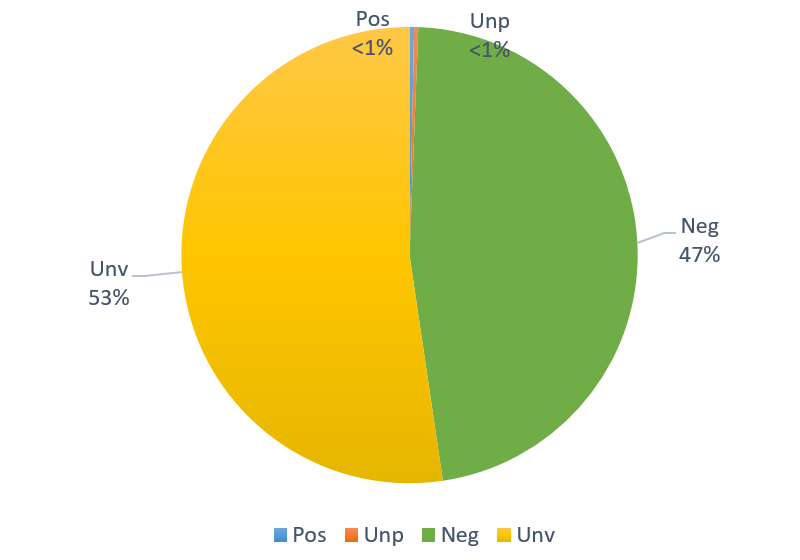
\includegraphics[width=7.9cm]{images/fan2.png}
		\caption{Lab Status}
	\end{minipage}
\end{figure}

\textbf{\subsection{Handle Null or Abnormal Values}}
In the 2021mcmproblemc\_dataset.xlsx file, you can easily find and fill in blank values using the Excel search function.Three NULL values can be found after sorting from smallest to largest by Detection Date.They should be excluded due to lack of time information.

There are also cases where Notes are empty in the table, with about 500 Notes rows out of 4,000 rows of data.This is because people only upload pictures when they upload information. These items can be further judged through image processing, so they are retained.

After sorting Detection Date, it can be found that the time format of some rows is MM/DD/YY, which is different from the majority of rows in the table. In addition, the time of these rows is before 1900, and they are outliers. Therefore, these rows are excluded in the screening process.

The latitude and longitude provided in the table were detected and found to be within a reasonable range. The latitude and longitude in the map drawing table intuitively showed that the points were all within the range of Washington State.

\begin {figure}[h]
\centering
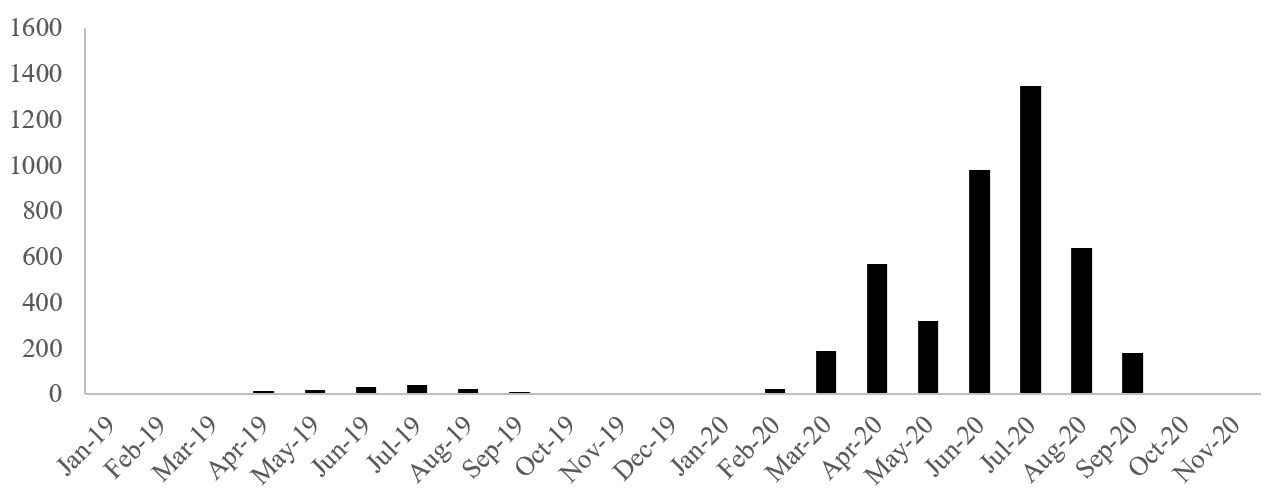
\includegraphics[width=14cm]{images/tiao.png}
\caption{Number of Reports}
\end {figure}

\textbf{\subsection{Remove Useless Data}}
By observing the sorted years, it can be found that most of the spots were found between 2019 and 2020, of which the latter accounted for the vast majority.There are only about 50 data before 2019, and these data are not of great analytical value because the years are too scattered, so they are excluded from these years.


According to statistics, among all the 3305 picture documents, there are 3111 JPG files, accounting for the vast majority of all the documents. The other files have various formats, which are not easy to be processed uniformly, and some of them also include text information, so they are directly removed.

Add a new column to 2021mcmproblemc\_dataset.xlsx. If a JPG file exists, it will be the file name. If no JPG file exists, the column will be blank.

% ----------------------------------------------------
% Section 3
% ----------------------------------------------------

\textbf{\section{Prediction}}
\textbf{\subsection{Examination}}
As the start point for further research, the spread of hornets should be to related to time. The first problem here is how to use data to represent the spread of hornets. we use time series analysis to examine this time series is a weak stationary process and this value is relavant to time. The amount of hornet sighting is adopted to illustrate the increasement of hornets amount, so the amount variation of hornets by time is discuessed. However, since the amount of positive samples are 0 is common in each month, it's not suitable to discuss this varietion in month. On the other hand, it's still unreachable to see the variation in years since the data only mainly include two years. Under the comprehensive consideration of the Seasonal habits of hornets as the profile said, using quarter (three months) as the time window to have an effective statistics (Figure \ref{1}). So divide 2019.01-2020.12 into 8 quarters.

\begin {figure}[h]
	\centering % 居中显示
	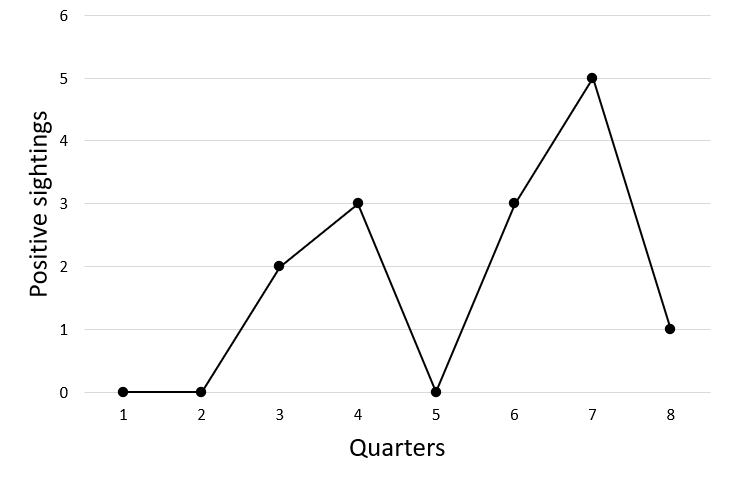
\includegraphics[width=11cm]{images/1.png}
	\caption{Number of Positive Sighting by Quarters}
	\label{1}
\end {figure}

\textbf{\subsubsection{Stability Test}}
First, we examine stability of this time series, using augmented Dickey–Fuller test (ADF).\cite{bib3} 

Hypothesis: $H_{0}: |\rho| \geqslant 1, H_{1}: |\rho| \textless 1;$ $H_0$ represents the series is stationary and $H_1$ represents the series is not stationary.

Test statistic: $$t = \frac{\hat{\rho}- 1}{\hat{\sigma_p}}$$

After the calculation of test statistic $t$, and designating the confidence level, the probability of $t$ in the confidence interval (CI) could get by seeking existed table. Another method is calculate the probability of test statistic $t$ not in the CI, $p-value$. If this value is far less than confidence level $C$, it is considered $H_0$ is true with sufficient confidentce, or it is considered $H_1$ is true.

Let confidence level $C$ be 0.05, after calculated the $p-value = 0.846$. Since $p-value$ is far greater than confidence level, the series is related to its own history. In other words, the data of each moment is related to the historical data.

\textbf{\subsubsection{Correlation}}

The time is regarded as the independent variable and the number of sightings as the dependent variable, and the correlation is directly calculated.\cite{doi:https://doi.org/10.1002/0471667196.ess5050.pub2}

After calculation, $p-value = 0.167$, far greater than 0.05 of confidence level. And the correlation level $C = 0.540$, shows a moderate positive correlation between the two.

\textbf{\subsection{Prediction Method}}
\textbf{\subsubsection{Area Division}}
Cellular automata (CA) is mainly used to predict the spread of hornet. To use this method, the map is needed to be divided up to Cellulars before further process. We divide the area in this way:

\vspace{.3cm}
\begin{itemize}
	\item The rectangular area of 45° N to 50° N and 120° W to 130° W is taken as the research object.
	\item Latitude and longitude are drawn every 0.2 degree, dividing the graph into small rectangles.
\end{itemize}

According to HaverSineg equation of spherical distance

\begin{equation}
haversin(\frac{d}{R}) = haversin(|\varphi_2 - \varphi_1|) + cos(\varphi_1) cos(\varphi_2) haversin(\Delta\lambda)
\end{equation}

$$ haversin(\theta) = sin^2(\frac{\theta}{2}) = \frac{1-cos\theta}{2} $$

\vspace{.5cm}
Here, $R$ is the redius of earth, $\varphi_1$ and $\varphi_2$ is the latitude of two points and $\Delta\lambda$ is the absolute value of the difference between the longitude of two points.

In this way, the division ensures that the center of one rectangle is about 20\textasciitilde30 km away from the eight adjacent rectangles, which is the maximum distance that a fertilized female can fly.

\textbf{\subsubsection{Cellular Automata}}
Our cellular automata consists of the following elements:

\vspace{.3cm}
\begin{itemize}
	\item Space: Two-dimensional grids on the map.
	\item State: The state of each grid is defined as $s_{i, j}$, which represents the number of active nests of hornet in each grid.
	\item Neighbor: The neighbors of a certain cell are defined as its 8 adjacent cells.
	\item Evolution rules: The rules of evolution can be summarized as
	$$ s_{i, j}^{t+1} = f(s_{i, j}^{t}, s_{neighbor_{ij}}^{t}) $$
\end{itemize}

Assuming that the flight distance of the female hornet obeys Poisson distribution, the eight orientations of the flight process are equal-probability. \cite{WHITE2007193} Because the probability of the Poisson distribution is maximized around parameter $\lambda$, $\lambda = \frac{30 + 0}{2}$, meaning in the best condiction it fly 30 km away, and in the worst consition it only fly hundreds of meters away, which is rounded to 0 km. At the same time, the population limit of hornet within a grid is mainly dependent on latitude and can be simply assumed to be linearly negative.\cite{bib1} At the same time, suppose that an hornet produces a total of $eggs$ during the breeding period, and the probability of each egg successfully hatching is $alive\_prob$. Here, according to the history record, let $eggs = 20000$, $alive\_prob = 0.00001$ and the probability that a female hornet is fertilized is $fert\_prob = 0.35$.\cite{bib2}

\vspace{3pt}

Evolution rules:

\begin{itemize}
	\item $ 0 \leqslant s_{i, j} \leqslant limit $ 
	\item Only the influence of 8 cells around one cell and its own state on the next state is considered. Since the distance between neighbor cells in the south, east, north and west is slightly different from that of neighbor cells in the southeast, northwest, northeast and southwest, their contributions are considered separately. Note that the probability of female hornets flying along the south, east, north and west directions without flying out of the current grid is $p_1$, the set of neighbors in these four directions is $S_1$, and the probability of female hornets flying along the southeast, southwest, northeast and northwest directions without flying out of the current grid is $p_2$, the set of neighbors in these four directions is $S_2$.
	
	\begin{equation}
	\begin{split}
	s_{i, j}^{t+1} = fert\_prob \cdot eggs \cdot alive\_prob & \\
	\cdot \Big( s_{i, j}^t \cdot (p_1 + p_2) + 0.125 & \sum_{k=1}^{2}(1-p_k) \cdot \sum_{(i, j) \in S_k}s_{i, j}^t \Big) 
	\end{split}
	\end{equation}

\end{itemize}

\textbf{\subsection{Result}}

We use these sightings reported in 2019 as our initial data and assume that each report site has only one active hive at fitst.

\begin{table}[h]
	\centering
	\vspace{10pt}
	\begin{tabular}{>{\centering\arraybackslash}p{25em}}
		\toprule % 绘制第一条线
		Global ID \\ \midrule
		\{5AC8034E-5B46-4294-85F0-5B13117EBEFE\} \\
		\{5EAD3364-2CA7-4A39-9A53-7F9DCF5D2041\} \\
		\{124B9BFA-7F7B-4B8E-8A56-42E067F0F72E\} \\
		\{F1864CC3-508C-4E60-9098-B158AB413B03\} \\
		\{7F3B6DB6-2ED4-4415-8DC2-3F03EC88F353\} \\
		\bottomrule
	\end{tabular}
	\caption{Positive Reports in 2019}
\end{table}

\begin{figure}
	\centering
	
	\subfigure[2020-2023]{
		\begin{minipage}[b]{0.2\linewidth}
			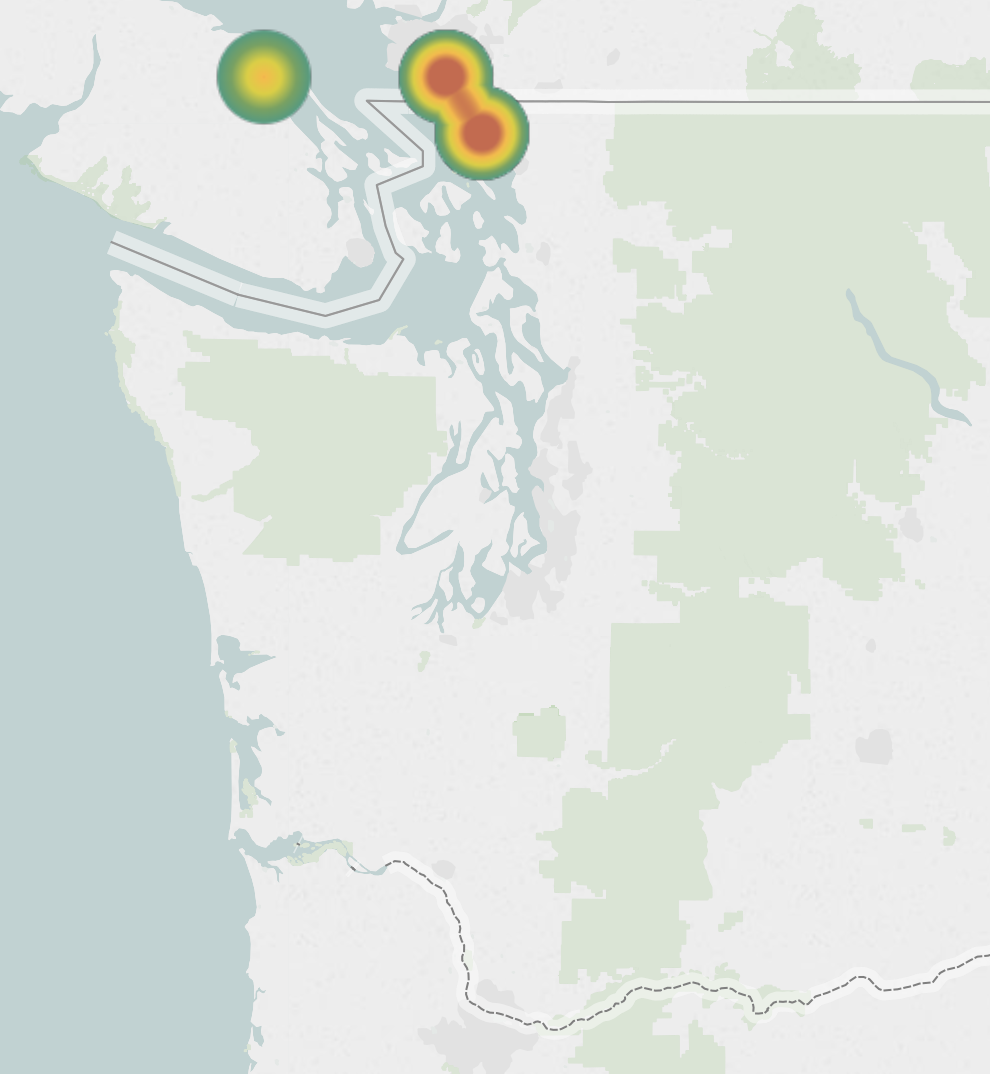
\includegraphics[height=3.2cm]{images/2020.png}
			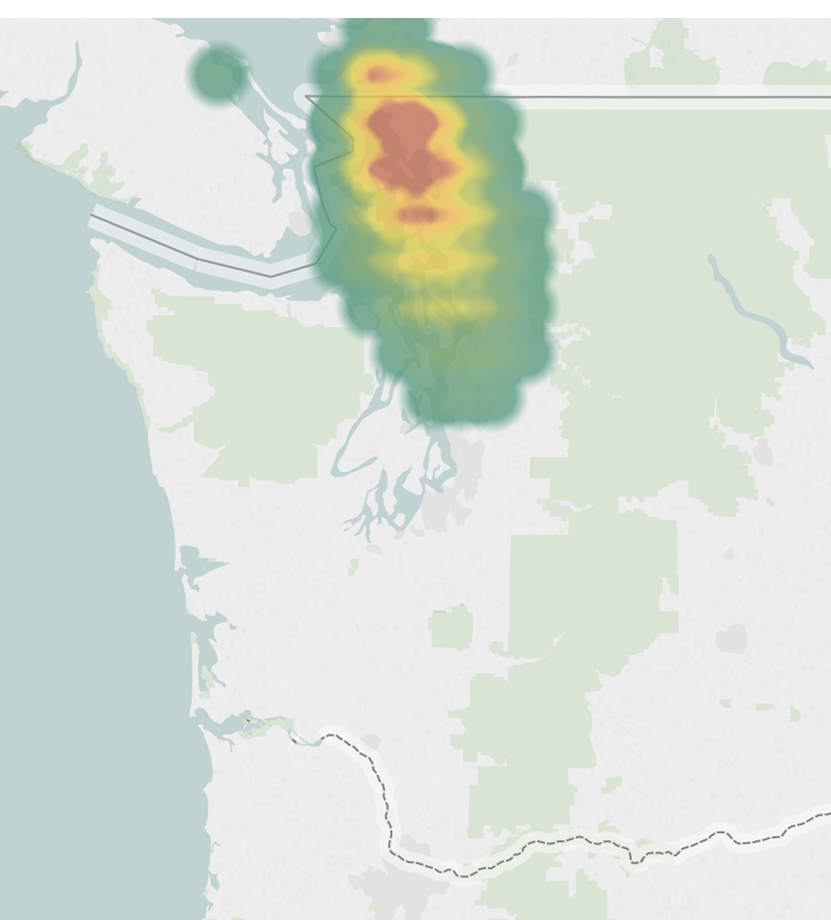
\includegraphics[height=3.25cm]{images/2022_1.png}
		\end{minipage}
	
		\begin{minipage}[b]{0.2\linewidth}
			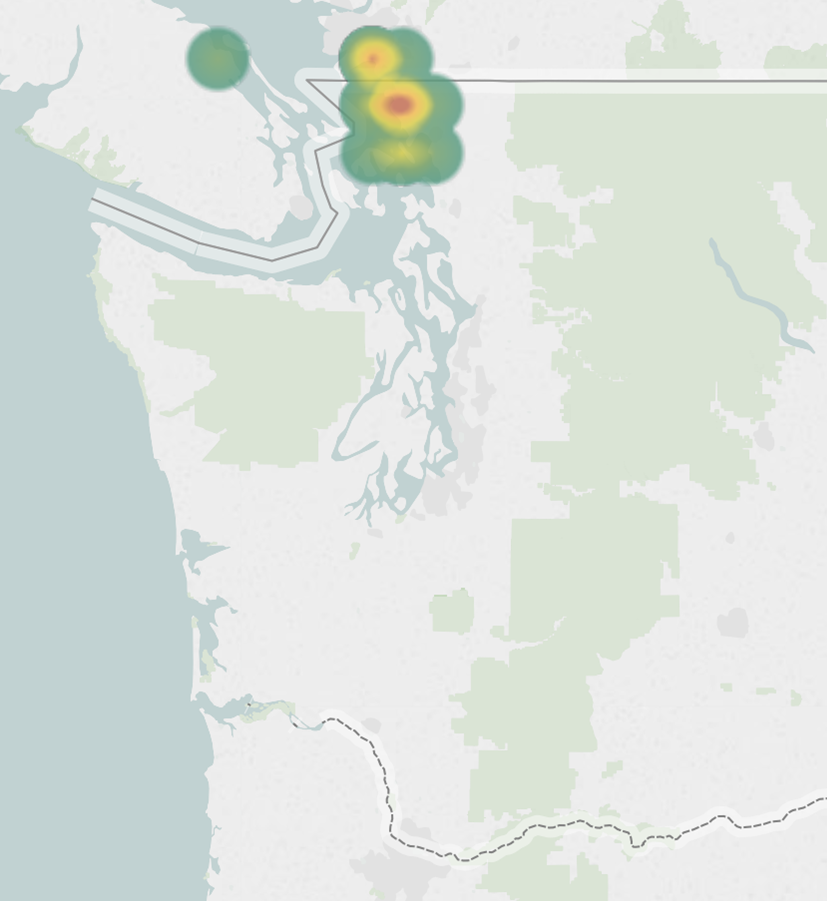
\includegraphics[height=3.2cm]{images/2021.png} 
			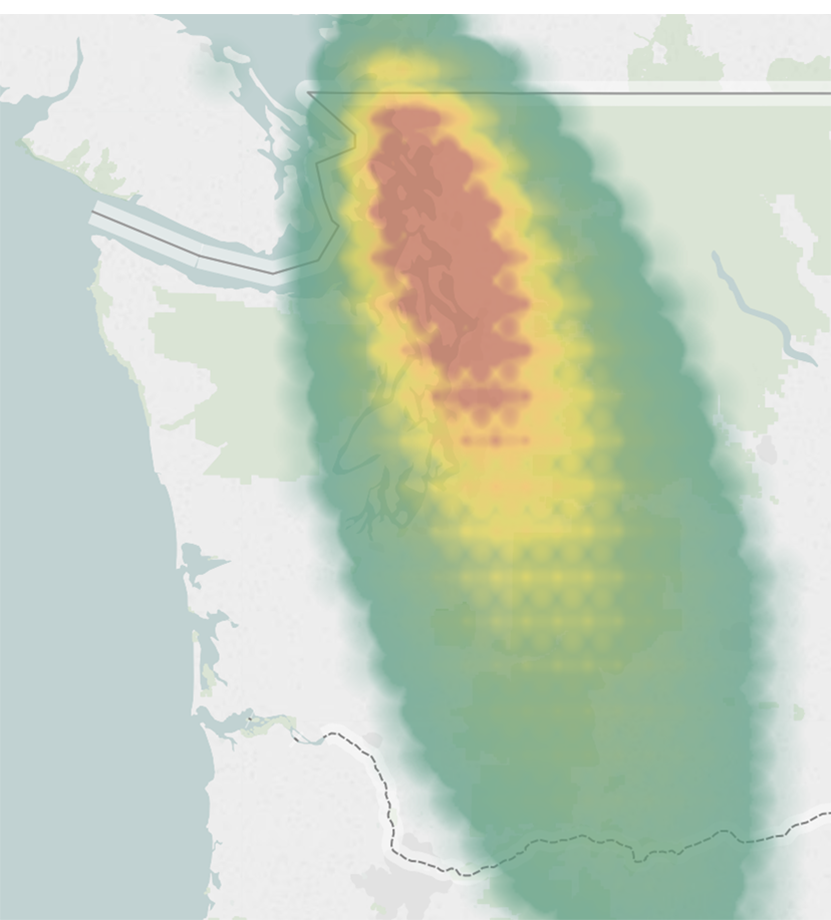
\includegraphics[height=3.25cm]{images/2023_1.png}
		\end{minipage}}
	\subfigure[2024]{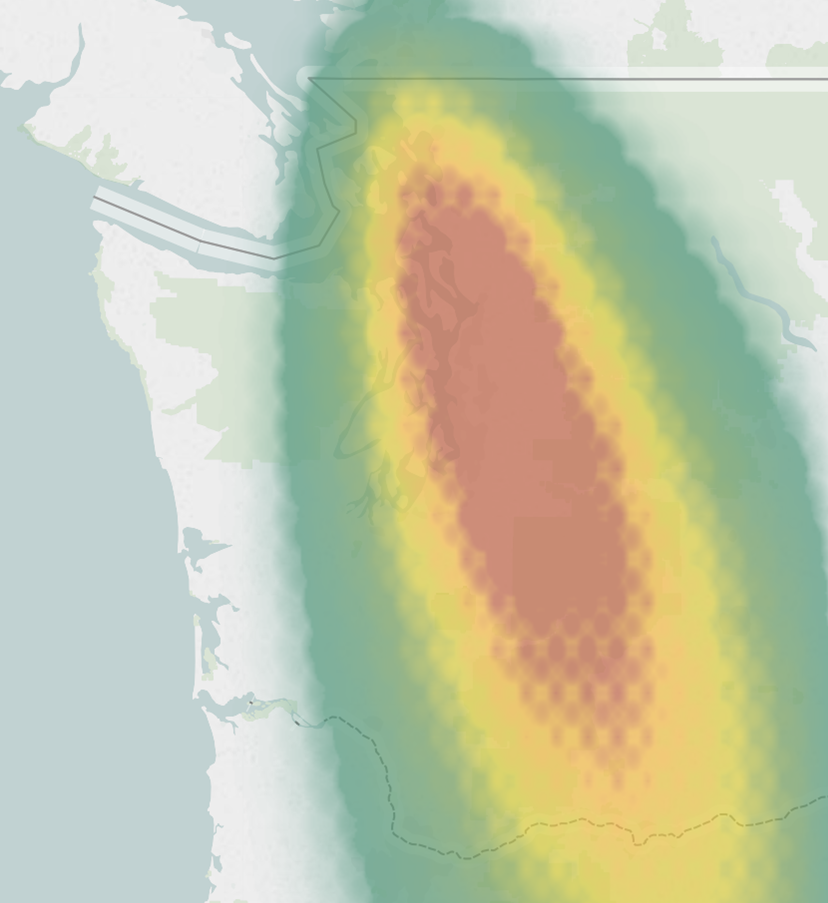
\includegraphics[height=6.5cm]{images/2024.png}}
	\caption{Prediction}
\end{figure}

It can be seen from the predicted results that the initial population size and the area involved were small, but with the passage of time, the population increased rapidly and the range expanded rapidly, which is in line with the characteristics of rapid spread of invasive species.By 2024, the western part of Washington state is almost completely lost, with a trend of rapid growth in the central part.In some areas, population of Asian giant hornets could reach more than 1,000. This is because high latitude largely limits the maximum population in each grid, which makes the population size in high latitude grows more slowly than that in low latitudes, resulting in a situation that the south is fast and the north is slow.

% ----------------------------------------------------
% Section 4
% ----------------------------------------------------

\textbf{\section{Model Constrction}}
\textbf{\subsection{Overview of Our Model}}

We selected the most important attributes from the report as our hierarchy (Figure 6). Then The problem is divided into four subquestions.

\begin {figure}[h]
\centering % 居中显示
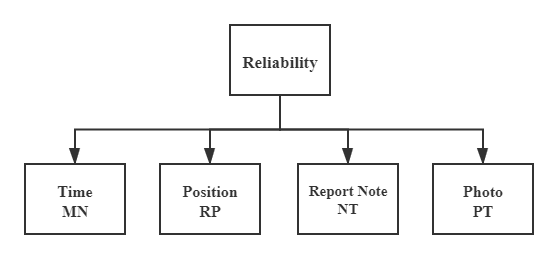
\includegraphics[width=12cm]{images/d.png}
\caption{Hierarchy of the Model}
\label{1}
\end {figure}

\textbf{\subsection{Subquestions with Submodels}}

\textbf{\subsubsection{Detection Time}}
For dection time, the main consideration is the probability of correct sighting reports of each month.Here, starting from the reverse side, calculate the probability of negtive sighting reports, $P_w$, and the probability of being positive, $P_r = 1 - P_w$.

We take negtive reports for each of the last two years, with respect to the frequency distribution of the months, because there are too few correct samples. The frequency is used as an estimate of the total error probability. Notice the data in the PDF attached points out that population is at its peak in August. In addition, there is also a case of correct sightings in winter. According to the data, except for the female hornets that survive the winter, the rest are basically dead in the winter. 

Considering that there will be 100\% false positives in a certain month, it is not accurate to estimate only through the original data. Therefore, data smoothing is needed. In reference to the hornet life cycle, the probability of sightings is lower in winter and higher in other seasons, so there is the following data smoothing strategy:

Note that the number of wrong samples for the $j$the month within two years is $W_j$, the number of correct samples is $R_j$, the total sample number is $T_j$, and the probability of reporting an error is $P_j$. Let


$$ max_w = max\{W_j\} $$
$$ max_r = max\{R_j\} $$
$$ min_w = min\{W_j|W_j > 0\} $$ 
$$ min_w = min\{R_j|R_j > 0\} $$

\begin{equation}
	W_j =
	\begin{cases}
		W_j + max_w & \text\{j \in 1, 2, 12\} \\
		W_j + min_w & \text\{j \in 3, 4, 5, 6, 7, 8, 9, 10, 11\}
	\end{cases}
\end{equation}

\begin{equation}
	R_j =
	\begin{cases}
		R_j + max_r & \text\{j \in 1, 2, 12\} \\
		R_j + min_r & \text\{j \in 3, 4, 5, 6, 7, 8, 9, 10, 11\}
	\end{cases}
\end{equation}

$$ T_j = W_j + R_j $$

results are as follows:

\begin{table}[h]
	\centering
	\vspace{10pt}
	\setlength{\tabcolsep}{7mm}
	\begin{tabular}{lllll}
		\hline % 绘制第一条线
		j  &$W_j$&$R_j$&$T_j$&$P_j$   \\ \hline
		1  & 715 & 1  & 716 & 0.9986  \\
		2  & 715 & 1  & 716 & 0.9986  \\
		3  & 6   & 6  & 12  & 0.5     \\
		4  & 43  & 6  & 49  & 0.87755 \\
		5  & 129 & 8  & 137 & 0.94161 \\
		6  & 186 & 7  & 193 & 0.96373 \\
		7  & 539 & 6  & 545 & 0.98899 \\
		8  & 715 & 7  & 722 & 0.9903  \\
		9  & 354 & 12 & 366 & 0.96721 \\
		10 & 88  & 8  & 96  & 0.91667 \\
		11 & 2   & 7  & 9   & 0.22222 \\
		12 & 714 & 2  & 716 & 0.99721 \\ \hline
	\end{tabular}
	\caption{Positive Reports in 2019}
\end{table}

According to the information provided, we can know that the probability of each negtive report error should approximately decrease and then increase with time, which corresponds to the first reproduction of hornet population in its life cycle (As the number of individuals in the population increases, the probability of being found increases), And population extinction (the number of individuals decreases, and the probability of being found decreases). Here, we choose a polynomial function to hit the variation process, using the Least Squares Method. After testing the 1-5 degree polynomial function, we finally decided to use the quartic function to fit the curve of reporting the change of error probability over time.

\begin{equation}
	P_w(m) = 0.0011m^4 - 0.0306m^3 + 0.2793m^2 - 0.9373m + 1.7591
\end{equation}

\begin {figure}[h]
	\centering % 居中显示
	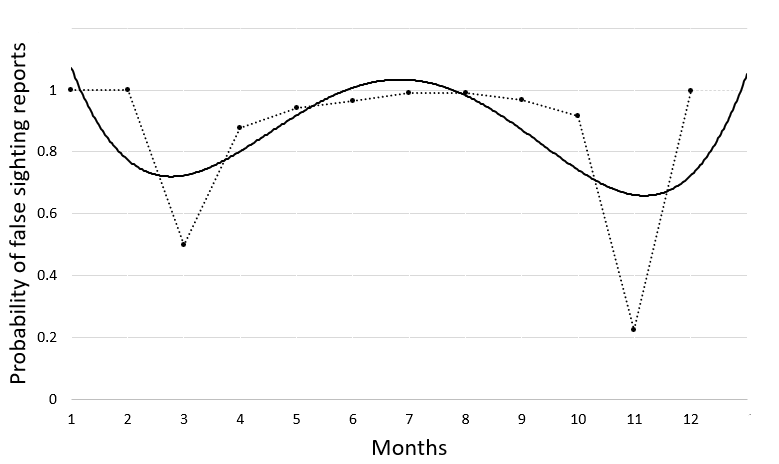
\includegraphics[width=11cm]{images/3.png}
	\caption{Frequent Words}
	\label{1}
\end {figure}

The two minimum points of the curve are March and November, respectively, which correspond to the time when hornets are awake and when they are out looking for nests, respectively, and tend to produce the most credible reports.

To fit the curve better, an extra abscissa is set, and the corresponding ordinate is the January value.It represents the estimated value on December 31, which should be close to the estimated value on January 1. In addition, it is observed that there are parts of the curve greater than 1, which will be replaced by a probability of 0.99.

\textbf{\subsubsection{Notes}}
To deal with Note, the first thing is converting each the note sentences to a numerical fixed-length vector. To get these vector, we pay attention to the importance to each words, using TF-IDF (Term Frequency / Inverse Document Frequency) \cite{7007894} to get calculate each important of words. Finally \_

TF represents the frequency of occurrence of word $w$ in sentence $D_{i}$. the $count(w)$ representes the the number of word $w$ in sentence $D_{i}$ and $|D_{i}|$ represents the number of words in sentence $D_{i}$.

\begin{equation}
	TF(w, D_{i}) = \frac{count(w)}{|D_{i}|}
\end{equation}

%Becaues we need to pick up important words in the whole notes but not in each single comments, we calculate the TF of words in the equation below. Operation $\sum_{i}$ means calculate the sum of $TF(w, D_{i})$ where $D_{i}$ contains words $w$ and $count(D_{i}, w)$ means the number of sentenses that contains word $w$.
%
%\begin{equation}
%	TF(w) = \frac{\sum_{i}^{}TF(w, D_{i})}{count(D_{i}, w)}
%\end{equation}

IDF reflects the prevalence of words. When a word is more common, this word has lower $IDF$ value. 

\begin{equation}
	IDF(w) = \ln{\frac{N}{1 + \sum_{i=1}^{N} I(w, D_{i})}}
\end{equation}

Then for any notes, we could calculate a TF-IDF vector to represent this notes. we use this value to measure the possibility in the note part in the following method: find the closest positive in Eular distance $d$

\begin{equation}
	d(x, y) = \sqrt{\sum_i(x_i - y_i)^2}
\end{equation}

We use the k-top frequent words to build a dictionary bu the statistics of all notes. After suspending of some meaningless words, we use k as 100 here and part of the dictonary are as below

\begin {figure}[h]
	\centering % 居中显示
	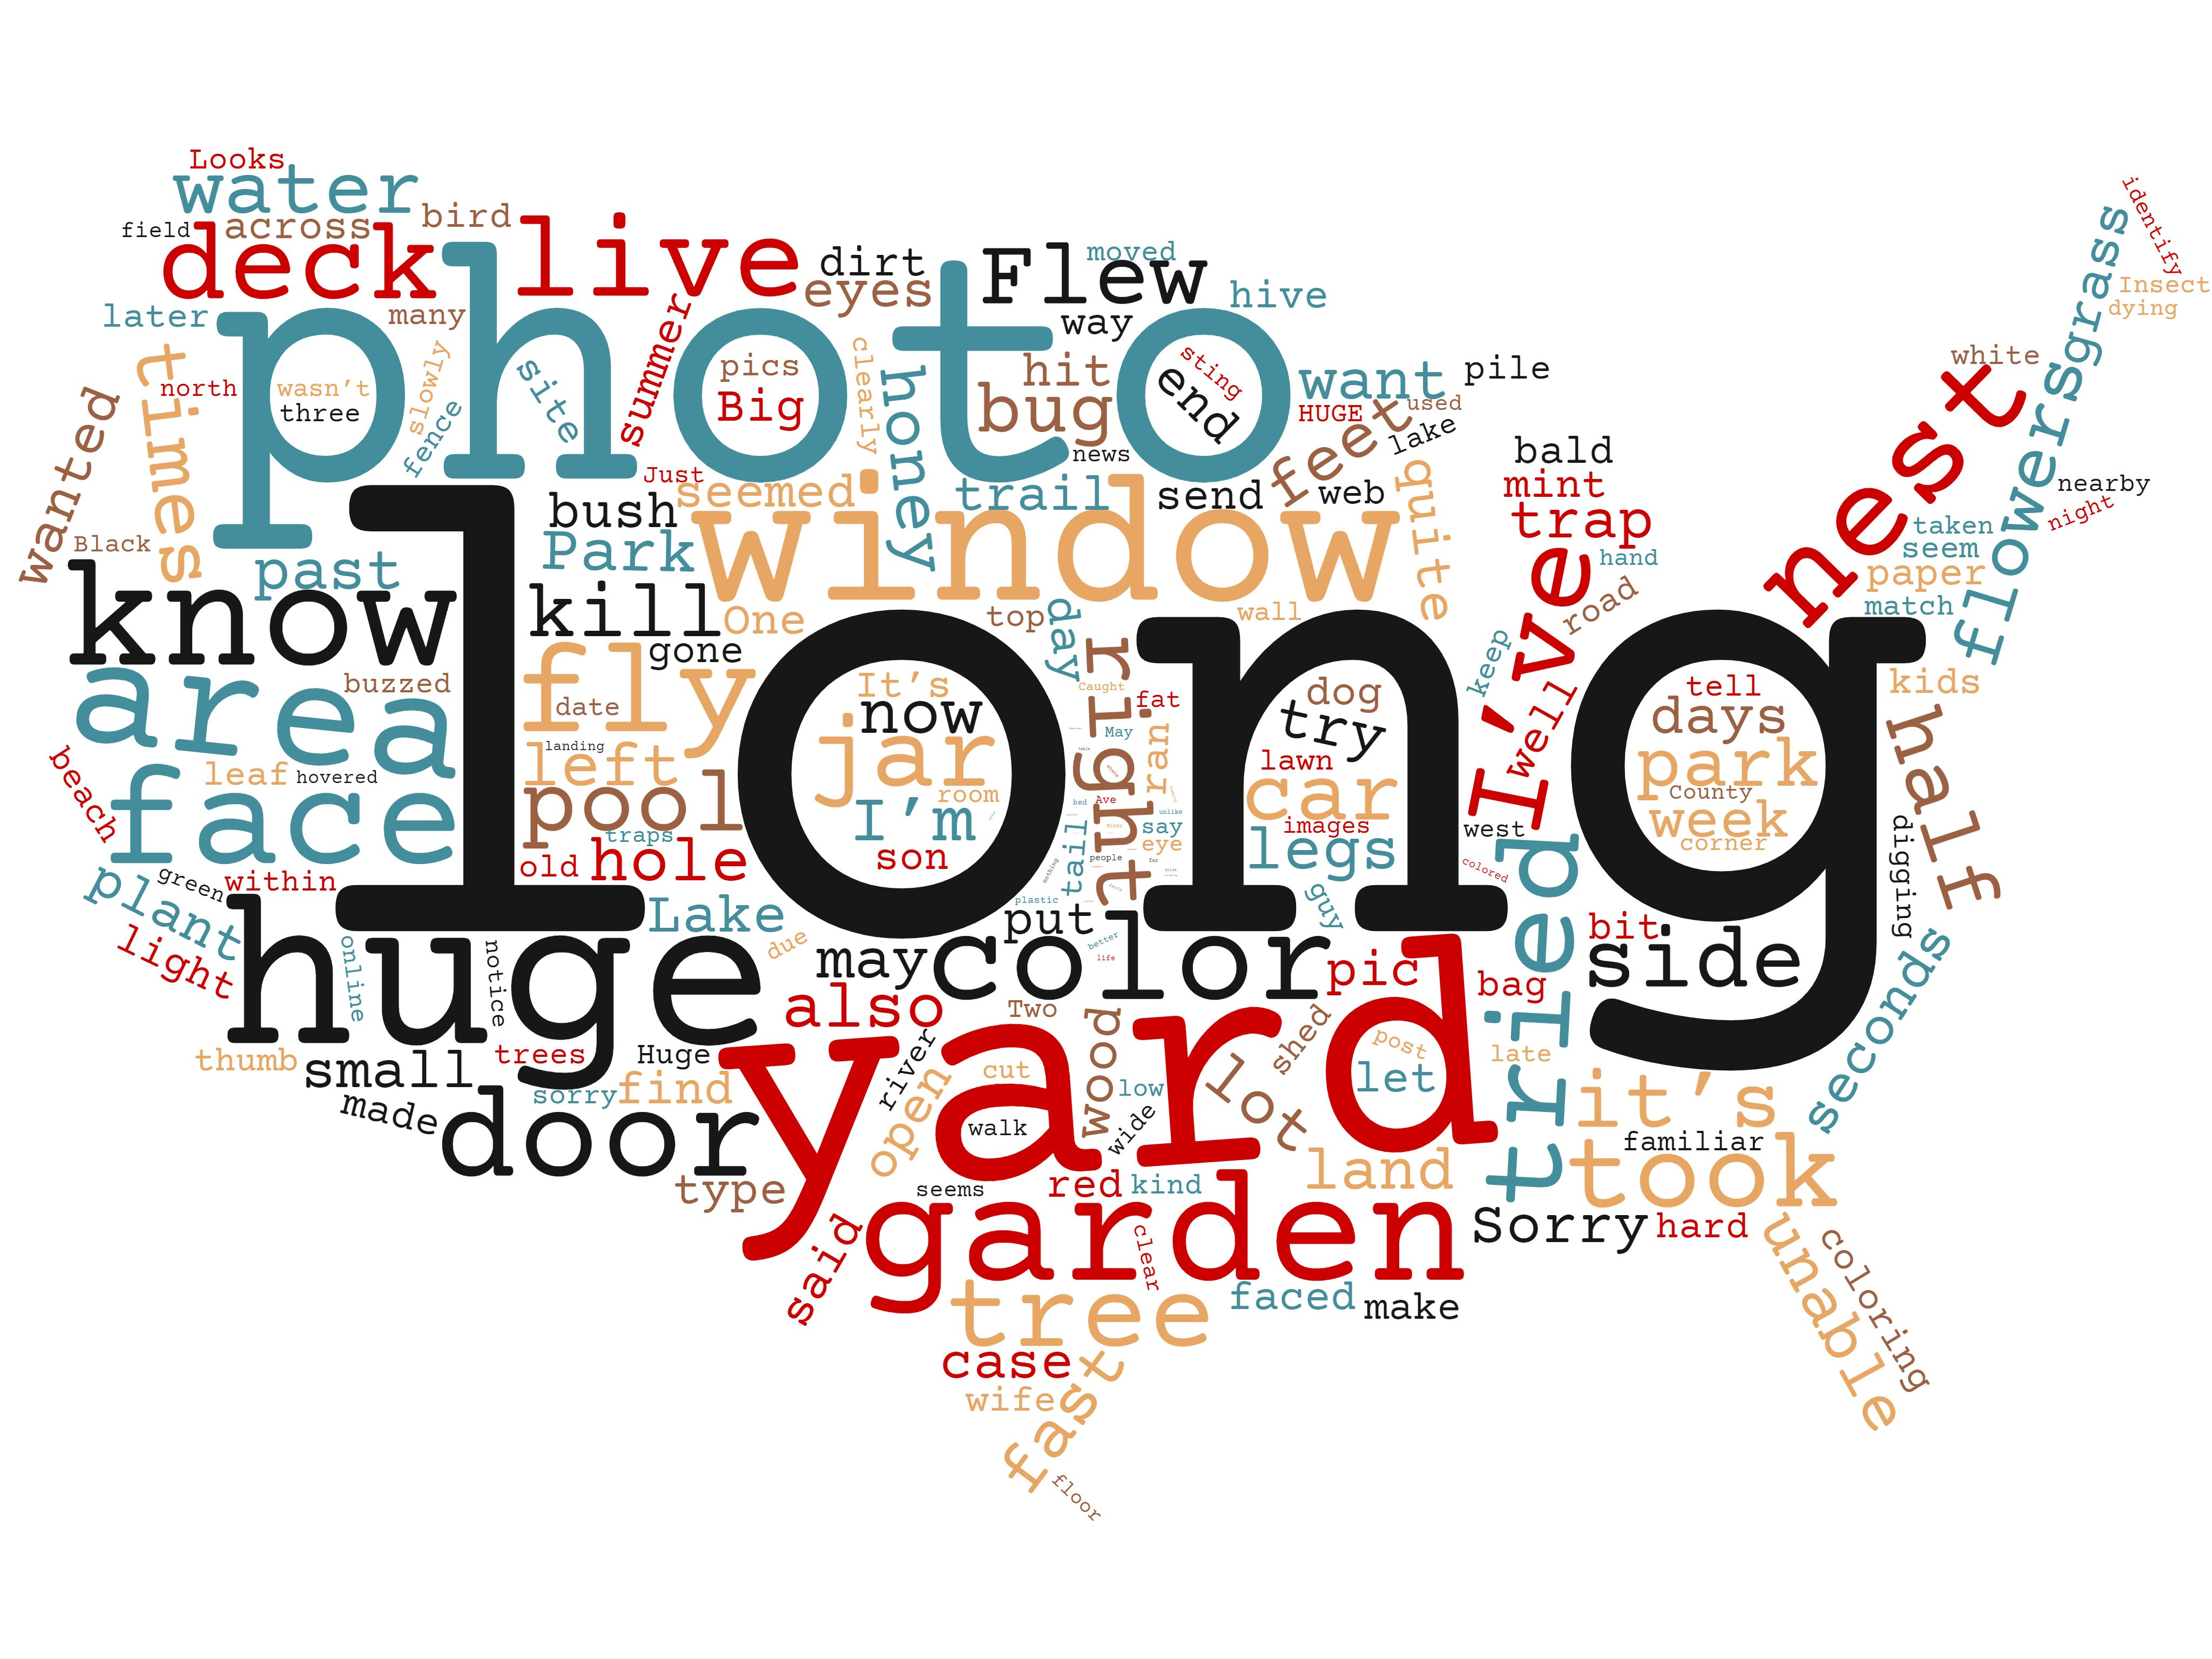
\includegraphics[width=11cm]{images/dic.jpg}
	\caption{Most Frequent Words}
	\label{1}
\end {figure}

In all the already curtain note, which already has the positive or negtive lab status, we pick up the cloest positive one and calculate the distance $d_{min}$, Finally, getting the $[0, 1]$ value of the note part.

\textbf{\subsubsection{Location}}
Still, we find the closet positive report and use the distance in sphere to calculate the distance $x$. Considering the America continent is big enough and the data is provided in latitude and longgitude, we calculate the distence between two sites in the radian system. The process of calculation is as below.

...

Then we get the closet positive distance $x$, and put this value in the function below, especially when the distance reach 30 km, this value should be very low since the information says hornets are hardly to reach 30 km away to build the nests. So we use a S shape function to dipict this trend.

Can we use another derivative to deal with the baseline function?

attach a photo of only this value here

\textbf{\subsubsection{Photographs}}

Image information is very important since..

a statictic of importance of imformation [image]

we could see image is a deterministic information to make sure if this specis is hornet.

We use cumputer methods to evaulate the image part and get a heuristic score. It's worth to say that because the pictures uploaded are various and have a lot of informations to deal with. It's hard to ecaluate by computer algorithm compeletly, so we introduce a human-in-the-loop method conbined with CNN to get the value of image.



% ----------------------------------------------------

\textbf{\subsection{the Determination of Weights}}
Using analytic hierarchy process (AHP) to assign weights, we need to consider the impact of month, feature description, and geographic location of the report. We compare the indicators with each other to build a comparative judgment matrix to represent the relative importance of the indicators, which is represented by $A$ below. After discussion, we think the importance is: photo, report location, month, and feature description.\cite{Shunsuke_Shiraishi1998KJ00001201864}

\makeatletter
\renewcommand*\env@matrix[1][\arraystretch]{%
	\edef\arraystretch{#1}%
	\hskip -\arraycolsep
	\let\@ifnextchar\new@ifnextchar
	\array{*\c@MaxMatrixCols c}}
\makeatother

\begin {figure}[h]
	\centering % 居中显示
	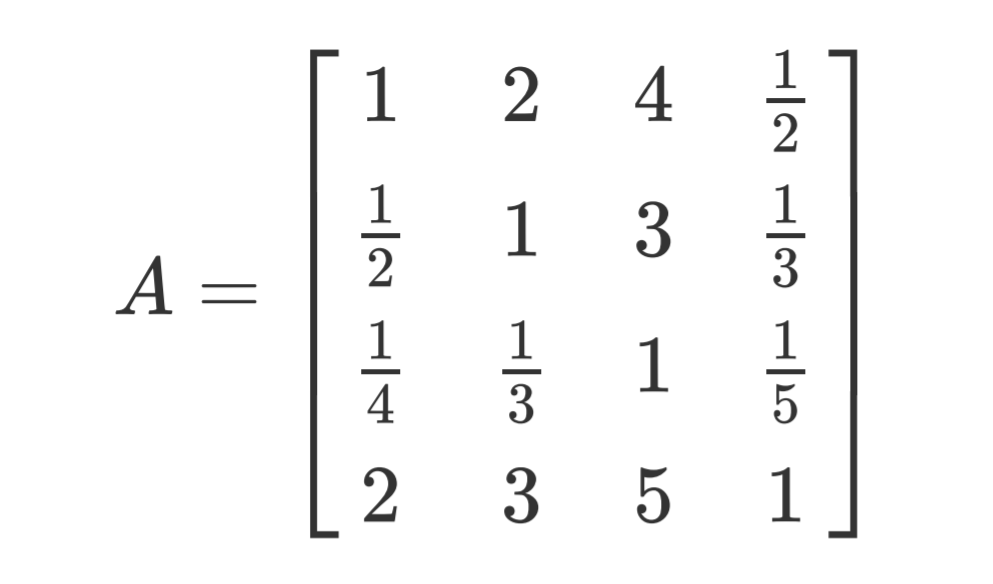
\includegraphics[width=6cm]{images/m.png}
\end {figure}

The larger the value of elements $a_{ij}$, the more important it is. $a_{ij}$ value greater than 1 means that the attribute represented by the i-th row is more important than the attribute represented by the j-th column.

The above matrix is a positive reciprocal matrix. According to the Perror theorem, it must have a maximum eigenvalue $\lambda\_max$, and the eigenvector $\vec{X}$ corresponding to $\lambda\_max$ is a positive vector. There is $AX = \lambda\_max \vec{X}$, All the components of $\vec{X}$ are unified for normalization, and the vector is obtained as the weight vector $\vec{W}$. After calculation, get $\lambda_max = 4.05111$ and 

$$ \vec{W} = [0.28438 \quad 0.16990 \quad 0.07286 \quad 0.47286 ] $$.

Then, the Reliability $R$ calculation formula is obtained.

\begin{equation}
	R = \vec{W} \cdot (RP, MN, NT, PT)^T
\end{equation}

\vspace{-20pt}

% ----------------------------------------------------
% Section 5
% ----------------------------------------------------

\textbf{\section{Model Simulation and Problem Solving}}
\textbf{\subsection{Task 1}}
Task 1 has already solved in section 2, Predicton.

\textbf{\subsection{Task 2}}
According to the report reliability evaluation system we established, we used our reliability analysis on the original Report data. It can be seen that most of the positive samples rank in the front after the reliability of each Report are estimated and ranked by our evaluation system. 

\begin{table}[h]
	\begin{tabular}{lllllll}
		\hline
		\multicolumn{1}{r}{\textbf{Global ID}}   & \multicolumn{1}{r}{RP} & \multicolumn{1}{r}{MN} & \multicolumn{1}{r}{NT} & \multicolumn{1}{r}{PT} & R    & Lab Status  \\ \hline
		\{5EAD3364-2CA7-4A39-9A53-7F9DCF5D2041\} & 1.00                   & 0.98                   & 1.00                   & 0.43                   & 0.73 & Positive ID \\
		\{49D016FA-358D-4BB0-9678-4F332DCBF3C6\} & 0.84                   & 0.73                   & 0.64                   & 0.62                   & 0.70 & Unverified  \\
		\{F1864CC3-508C-4E60-9098-B158AB413B03\} & 1.00                   & 1.00                   & 0.57                   & 0.35                   & 0.66 & Positive ID \\
		\{BEAC832C-0783-414A-9354-C297F38570AD\} & 1.00                   & 0.75                   & 1.00                   & 0.37                   & 0.66 & Positive ID \\
		\{5AC8034E-5B46-4294-85F0-5B13117EBEFE\} & 1.00                   & 0.75                   & 1.00                   & 0.37                   & 0.66 & Positive ID \\
		\{DEF5D82B-E326-41A5-9B6C-D46DCD86950C\} & 1.00                   & 0.72                   & 1.00                   & 0.35                   & 0.65 & Positive ID \\
		\{A717D86F-23E9-4C8C-9F12-198A71113E93\} & 1.00                   & 0.22                   & 1.00                   & 0.53                   & 0.64 & Positive ID \\
		\{AA461F47-1B2B-4EA1-8154-ECF70B55A334\} & 1.00                   & 0.70                   & 1.00                   & 0.35                   & 0.64 & Positive ID \\
		\{7F3B6DB6-2ED4-4415-8DC2-3F03EC88F353\} & 1.00                   & 0.73                   & 1.00                   & 0.34                   & 0.64 & Positive ID \\
		\{A0909E9E-FBC6-4DAA-9B25-D44C990A7B3B\} & 0.89                   & 0.93                   & 0.64                   & 0.35                   & 0.63 & Unverified  \\ \hline
	\end{tabular}
	\caption{Top 10 Results ranked by Raliability}
\end{table}

It can be seen from observation that a small number of positive samples are not in the list because of the absence of photos and other elements, which are within the range of explanation.

Back to our original question, to measure the possibility that a Report is misclassified, we only need to look at its reliability. If the reliability is low, the greater the probability that it is a negative Report; otherwise, if the reliability is high, the smaller the probability that it is a negative Report.

\textbf{\subsection{Task 3}}

For this problem, due to the limited manpower and material resources, it is a rational decision to prioritize the areas with high reliability of reports as the survey target. If there are multiple areas with high reliability, we choose the areas with more intensive distribution of reports as our survey target.All we need to do is find those areas where reliable reports are concentrated and prioritize them.We chose the lower quartile of the indicators of the positive sample as the threshold, and reports above this threshold were considered to have high reliability.For all reports whose reliability indicators are above the threshold regardless of their Status, we can see their distribution on the map:

\begin {figure}[h]
\centering
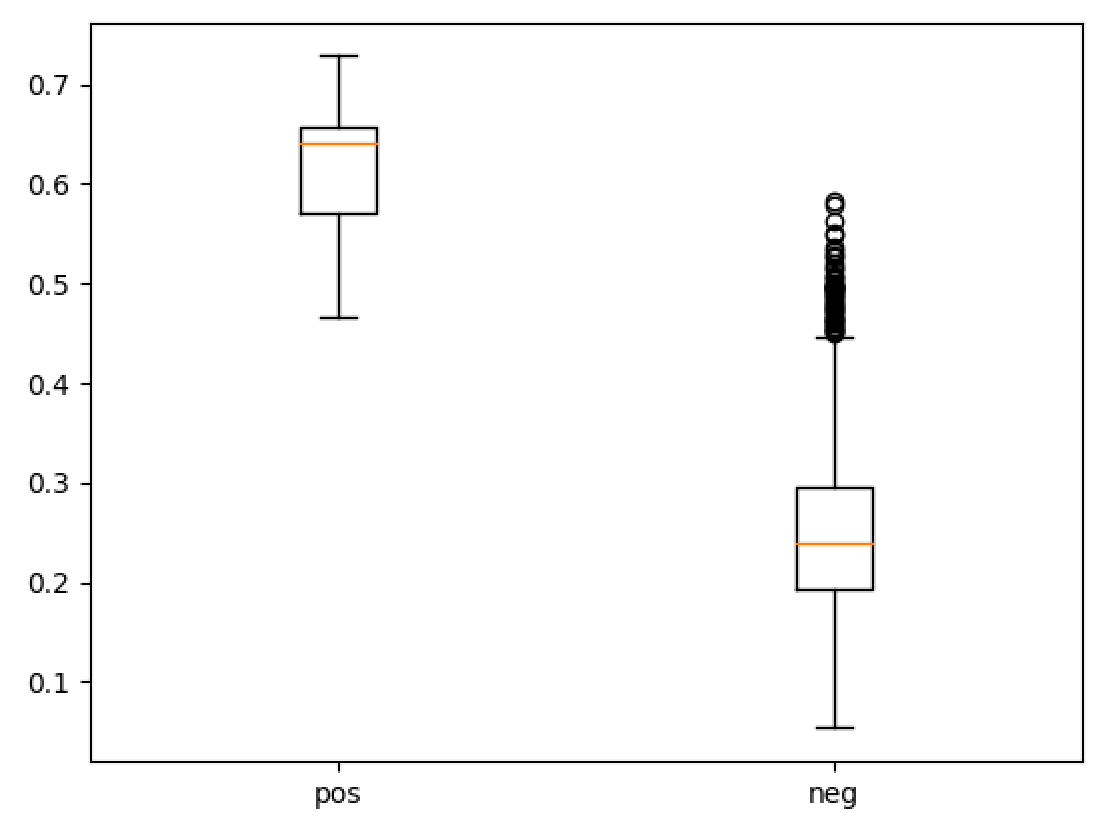
\includegraphics[width=8cm]{images/box.png}
\caption{Reliability of Prediction}
\label{key}
\end {figure}


\begin {figure}[h]
\centering
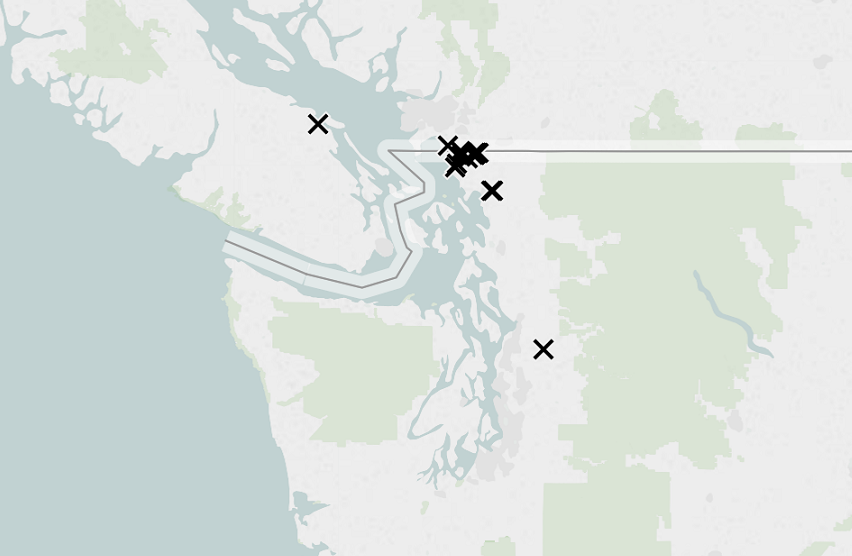
\includegraphics[width=10cm]{images/map.png}
\caption{Key Area}
\label{map}
\end {figure}

Therefore, give priority to the investigation of 49.0° N 122.7° W area (figure 7). It's near Bellingham city.

\textbf{\subsection{Task 4}}

From the model idea mentioned above, the model we built relies largely on positive report data.However, due to the absence of positive report data (only 14), the data of positive reports had a greater impact on our model than the addition of negative reports.Considering that the more data the more accurate, the model should be updated as frequently as possible. However, too frequent updating will bring unbearable calculation cost. Therefore, a balance between updating frequency and calculation cost should be achieved.

\begin {figure}[h]
\centering
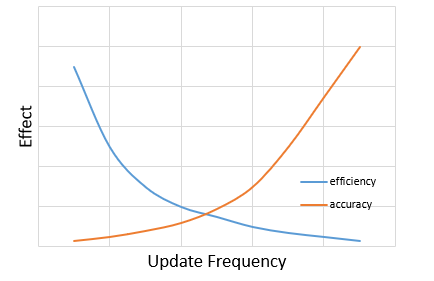
\includegraphics[width=9cm]{images/fork.png}
\caption{Change Rule}
\end {figure}

We assume that the new report we get has been confirmed by the laboratory whether it is hornet or not. If not, we use the current model for preliminary confirmation (if the reliability value is greater than the positive report, otherwise it is considered negative report).We adopt the following update strategy:

\begin{enumerate}[1.]
	\item Maintain a queue for a new report, which is initially empty.
	
	\item If no new positive reports appear, then we update our model about once a month.Update model including put the pictures of the new report added to the image recognition of neural network in the training set and the training of neural network further, recount each point to the nearest k report point distance and update the RP value, recount positive report along with the change of in relation to a new curve fitting, and the influence of back calculation note value.
	
	\item If new, more positive reports emerge, we immediately update the model.
	
	\item When the update is complete, clear the queue and wait for the next update.
\end{enumerate}

\textbf{\subsection{Task 5}}
Considering that hornet have a one-year propagation cycle, we chose one year as the time window for observation.

Let the set of all reports received in a certain region within a year starting from a certain month be $S_i$, The probability of a positive report for the month is measured by $p_i$, $p_i = max\{Reliability_r | r \in S_i \}$. As long as $p_i < \alpha$, we think it is unlikely that positive samples will be available this month, and therefore that hornet will not be found, so we call this month "Safe".

But it depends a lot on the month we choose. In some months people send very few reports, and it is very likely that all the reports they receive match the missing photos or missing comments, leading to the false impression of a lower indicator.But through the analysis of the data before it is known that people report number downturn will not more than 6 months, so we just need to continue to examine the possibility of positive report every month within six months, 6 months as long as it is "safe", so we think the probability of the region found Asian hornet is extremely low, can think Asian hornet has been eliminated in the region.

% ----------------------------------------------------
% Section 6
% ----------------------------------------------------

\textbf{\section{Model Analysis}}

The sensitivity of our model mainly comes from our determination of the weight of each factor in the index. Therefore, we change the weight of each component respectively to observe its influence on the results of analyzing the topic data of our model.

\begin {figure}[h]
\centering
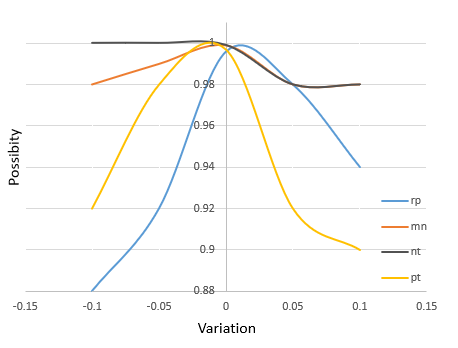
\includegraphics[width=11cm]{images/min.png}
\caption{Sensibility}
\label{13}
\end {figure}

Therefore, the model is insensitive to time and locations, and relatively sensitive to notes and photos.

\textbf{\subsection{Model Sensitivity Test}}
The sensitivity of the model mainly comes from our determination of the weight of each factor in the index. Therefore, we changed the weight of each component respectively to observe its influence on the result of analyzing the topic data of our model.

\textbf{\subsection{Strengths}}
\begin{itemize}
	\item Rapid prediction
	\item Fast Iterative Update
\end{itemize}
\textbf{\subsection{Weaknesses}}
\begin{itemize}
	\item Recalculating the neural network is time-consuming
\end{itemize}

% 因为不输出此部分到目录 \addcontentsline{}{}{}是添加此标题到目录 
\newpage
\textbf{\section*{References}\addcontentsline{toc}{section}{References}}
\fancyhf{}
\fancyhead[R]{ }
\fancyhead[L]{ }
% \addbibresource{books.bib}
\bibliography{books.bib} %bibfile_name
\Large
\bibliographystyle{IEEEtran}

\end{document}